\documentclass[12pt]{article}
\usepackage[margin=1in]{geometry}
\usepackage{amsmath,amsthm,amssymb}
\usepackage{graphicx}
\usepackage{setspace}
\doublespacing

\title{New Methods for Studying Old Work}
\author{José Ignacio Velarde Morales}

\begin{document}
\maketitle
\tableofcontents

\section{Introduction}
  \subsection{Motivation for studying new work}
  \subsection{ML for econ}

\section{Related Literature}
  \subsection{Literature about new work}
  \subsection{NLP literature}
  \subsection{Econ and ML literature}

\section{Data}
  \subsection{Dictionary of Occupational Titles}
  The Dictionary of Occupational Titles (DOT) is a volume that was created by the United States Department of Labor to help match job openings and job seekers. It provides detailed textual descriptions of thousands of jobs. The job descriptions generally describe what work is done, who it is done by, and why it is done. The descriptions also include information regarding the industry and occupation group the job is in.

  \begin{figure}[h]
    \centering
    \caption{Example definition from the 1939 DOT}
    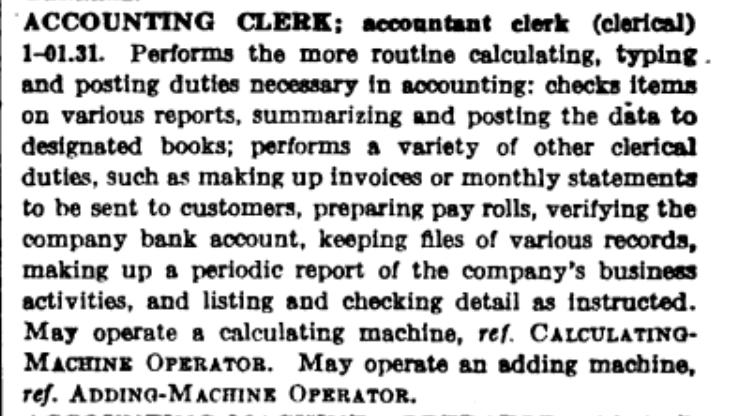
\includegraphics[width=0.6\textwidth, keepaspectratio=true]{images/dot_def}
  \end{figure}

  There are 5 editions of the DOT, published in 1939, 1949, 1965, 1977, and 1991. Each edition has about 20,000 job definitions. The 1965, 1977, and 1991 editions of the DOT include structured information about the jobs in addition to the textual description. The structured information is in the form of numerical codes that quantify job complexity, training requirements, and skill requirements. These codes are further described below.

  \subsubsection*{Data, People, Things Codes}
  Each job is assigned a 3-digit code that describes the job's complexity in relation to data, people, and things. Each digit in the code corresponds the job's complexity in one of those three categories. For example, the job of Aeronautical Test Engineer has a code of 061. The code tells us the job has high data complexity, medium/low people complexity, and high things complexity. The figure below shows the meanings of the different codes.

      \begin{figure}[h]
        \centering
        \caption{Explanation of Data, People, Things Code}
        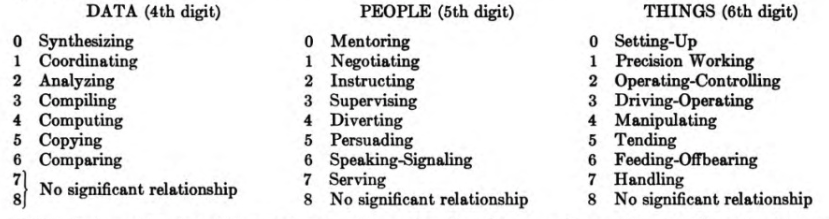
\includegraphics[width=0.95\textwidth, keepaspectratio=true]{images/DPT}
      \end{figure}

  \subsubsection*{Job Attributes}
  Job descriptions in the DOT include descriptions of the mathematical education, aptitudes, and temperaments required to perform each job. Mathematical education refers to formal and informal education that develops basic reasoning skills in math. Aptitudes are specific abilities that an individual should have in order to perform a specific job. Examples of aptitudes are finger dexterity and hand-eye coordination. Temperaments are adaptability requirements made on the worker by specific types of job situations. These can include directing activities or performing repetitive work. The full list of job attributes we predict can be found in the table below.
  % TODO: improve attributes description.

    \begin{table}[h!]
      \centering
      \begin{tabular}{|l|l|l|}
      \hline
      \textbf{Attribute}         & \textbf{Description}                                                   & \textbf{Scale} \\ \hline
      GED Math                   & Formal and informal education developing general math skills           & 1-6            \\ \hline
      Finger Dexterity           & Ability to use fingers to manipulate small objects                     & 1-5            \\ \hline
      Eye-hand-foot Coordination & Motor responsiveness to visual stimuli                                 & 1-5            \\ \hline
      Direct, control, plan      & Involves the direction, control and planning of activities & 0/1            \\ \hline
      Attain limits              & Involves the precise attainment of set limits or standards & 0/1            \\ \hline
      \end{tabular}
    \end{table}


  \subsection{1940 Census Complete Count Files (CCC)}
  The United States conducts a census every ten years to collect data about its population. The Census collects a wide range of information about respondents including occupation, income, education, race, and place of residence. The data is confidential, but becomes publicly available 72 years after Census Day. The data from the 1940 Census became publicly available in April of 2012.\\

  Many research projects that use Census data use the individual level micro data provided by IPUMS (cite?). One drawback
  of these micro data is that the occupational information in them is very coarse. For example, patent lawyers and divorce lawyers are both grouped into the occupation "lawyer". Each census occupation has a corresponding code. The complete count files have each respondent's written occupation in addition to their broad census occupation. Census occupations were assigned to respondents based on their written response. The written occupations often have typos and abbreviations. As a result, there are over 3 million unique job titles in the complete count files. The table below contains some sample written occupations.

  \begin{table}[h!]
    \centering
    \caption{Sample Occupational Titles from the Census Complete Count Files}
    \begin{tabular}{|l|l|}
      \hline
      \textbf{Occupation String} & \textbf{Census Occupation Code} \\ \hline
      Guard Fonman               & 602                             \\ \hline
      Operator Building          & 308                             \\ \hline
      Bank Runner                & 224                             \\ \hline
      Truck Winder               & 496                             \\ \hline
      Nutrinist                  & V52                             \\ \hline
    \end{tabular}
  \end{table}
  \FloatBarrier

  \subsection{1940 Census Alphabetical Index of Industries and Occupations (CAI)}
  The Alphabetical Index of Industries and Occupations is an official list of industries and occupations compiled by the US Census Bureau. It is continuously updated as occupations are created or become obsolete. The main purpose of the index is to map specific occupations into broader census occupation groups. The index was used by Census employees to assign respondents official census occupations and industries.

  \begin{table}[h!]
    \centering
    \caption{Sample Occupational Titles from the Census Alphabetical Index}
    \begin{tabular}{|l|l|}
      \hline
      \textbf{Occupation Title} & \textbf{Census Occupation Code} \\ \hline
      Bridge Inspector               & 318                        \\ \hline
      Buttonhole Marker          & 496                             \\ \hline
      Jewelry Polisher              & 436                        \\ \hline
      Inspector Oil               & 318                             \\ \hline
      Pattern Developer                  & 362                             \\ \hline
    \end{tabular}
  \end{table}
  \FloatBarrier

\section{Methods}
The main technical components of this project are matching job titles in the Census Complete Count Files (CCC)
to job titles in the Census Alphabetical Index of Occupations (CAI) and predicting job attributes
based on the textual descriptions of jobs in the 1939 Dictionary of Occupational Titles.

  \subsection{Documents as Vectors}
    \subsubsection{Bag of Words Representation of Documents}
      A corpus is a collection of documents, and documents are collections of words. One way to represent a document is a vector is the "bag of words" approach. In this approach, a corpus can be represented as a matrix where the rows represent documents and the columns represent words. The $i,j$th entry of this matrix corresponds to how many times word $j$ appeared in document $i$. For example, the corpus consisting of the two sentences: "The dog bit the cat" and "The cat bit the mouse" would be represented by the following term-document matrix where the columns correspond to the words the,dog,bit,cat,mouse.

        \begin{align*}
        \begin{bmatrix}
        2 & 1 & 1 & 1 & 0\\
        2 & 0 & 1 & 1 & 1\\
        \end{bmatrix}
        \end{align*}

        Note: that words that are too common, such as "the", are called "stop words" and are often excluded from term-document matrices. Words that appear in all documents are also excluded.

      \subsubsection{TF-IDF Weighing}
      TF-IDF weighing is a way to give more importance to words that are more meaningful. TF stands for "term frequency". This is how many times a word appears in a document. IDF stands for "inverse document frequency". This corresponds to the number of documents in the corpus the word appears in. The $i,j$th entry in the TF-IDF matrix will be $tf(j,i) \times idf(j)$ where $tf(j,i)$ is how many times word $j$ appears in document $i$ and $idf(j)$ is word $j$'s inverse document frequency. The matrix's rows are then normalized to have a Euclidean norm of 1.\\

       Words that are very common, such as "the", "and", or "because", will have a very large document frequency because they will appear in most documents. As a result, they will have a very small inverse document frequency and their importance will be decreased. The exact formula for inverse document frequency used is:

        \begin{align*}
          idf(w) &= \log{\frac{n}{1+df(w)}} +1
        \end{align*}
        \\
      where $n$ is the number of documents in the corpus and $df(w)$ is the number of documents word $w$ appears in.

    \subsubsection{RoBERTa}

  \subsection{Matching procedure}
    The procedure used to match titles in the CCC to titles in the CAI is summarized below and elaborated on in the following subsections. The table below also shows how the match rate evolves at each step.

    \begin{enumerate}
      \item \textbf{Preprocessing} remove capitalization, extra whitespace, and punctuation.
      \item \textbf{Exact Match} match observations with identical processed title and census occupation code.
      \item \textbf{Stemmed Match} match observations with identical census occupation code and identical stemmed job title.
      \item \textbf{Industry Info Match} concatenate job title and industry in the CAI and match to observations in the census with identical census occupation code and job title.
      \item \textbf{TF-IDF Match} match observations with identical census occupation code and TF-IDF score of over 0.70.
    \end{enumerate}

    \begin{table}[h!]
      \centering
      \caption{Matching Progression}
      \begin{tabular}{|l|l|l|l|}
      \hline
      \textbf{Method}     & \textbf{Match Rate} & \textbf{New Titles} & \textbf{New Workers} \\ \hline
      Exact Match         & 67\%                & 1328                & 209,931              \\ \hline
      Stemmed Match       & 68\%                & 1388                & 237,449              \\ \hline
      Industry Info Match & 68\%                & 1388                & 237,452              \\ \hline
      TF-IDF Match        & 83\%                & 2203                & 1,245,696            \\ \hline
      \end{tabular}
    \end{table}

    \subsubsection{Preprocessing}
      \begin{enumerate}
        \item Make all characters in the job title and census occupation code lowercase.
        \item Remove any non alpha-numeric characters in the job title.
        \item Remove any leading and trailing whitespace from both the job title and the census occupation code. Remove any extra whitespace between words in the job title. For example, "Patent \space \space \space Lawyer" becomes "Patent Lawyer".
      \end{enumerate}

    \subsubsection{Exact Match}
      Match observations with identical processed title and census occupation code.

    \subsubsection{Stemmed Match}
      The goal of stemming is to reduce words to their base form. For example the words: \textit{operate, operating, operated} would all be turned to \textit{oper}. In this part of the matching procedure, we stem all of the words in the job title using the Porter stemming algorithm. We then match observations whose stemmed job titles are identical and have identical census occupation codes. For example, an observation in the CCC with the occupation code "020" and job title "farm labor" would be matched to the CAI title "farm laborer" with occupation code "020".

    \subsubsection{Industry Information Match}
      We create another title in the CAI data by concatenating the processed job title and the processsed industry title. We then match observations in the census whose processed job title exactly matches the concatenated job and industry title in the CAI and that have the same occupation code.

    \subsubsection{TF-IDF Match}
      We treat job titles as documents and groups of job titles with the same census occupation codes as corpuses. So, for example, all of the job titles under occupation code "V12" would be one corpus and all of the job titles under occupation code "V70" would be another corpus. We then compute the TF-IDF weights for all of the words in the CAI job titles. Given a job title from the CCC, we match it to the job title in the CAI whose terms have the highest sum of TF-IDF weights as long as the sum is over 0.7 \\

      \textbf{Example:} The occupation code, "780: Waiters and waitresses" has the following titles in the CAI: 'waitress', 'waiter', 'counter man', 'soda clerk', 'hostess', 'dispenser soda water', 'head waiter', 'soda jerker'. An observation in the CCC with an ocupation code of 780 and a job title of "clerk" would be matched to "soda clerk" because the word "clerk" is very uncommon in job titles with occupation code of 780.

  \subsection{Prediction}

\section{Results}
  \subsection{Matching Rate/Validation}
  \subsection{Attribute Prediction}

\section{Conclusion}








\end{document}
